%\documentclass{standalone}
%\usepackage{tikz}
%\usetikzlibrary{patterns,plotmarks}
%\begin{document}
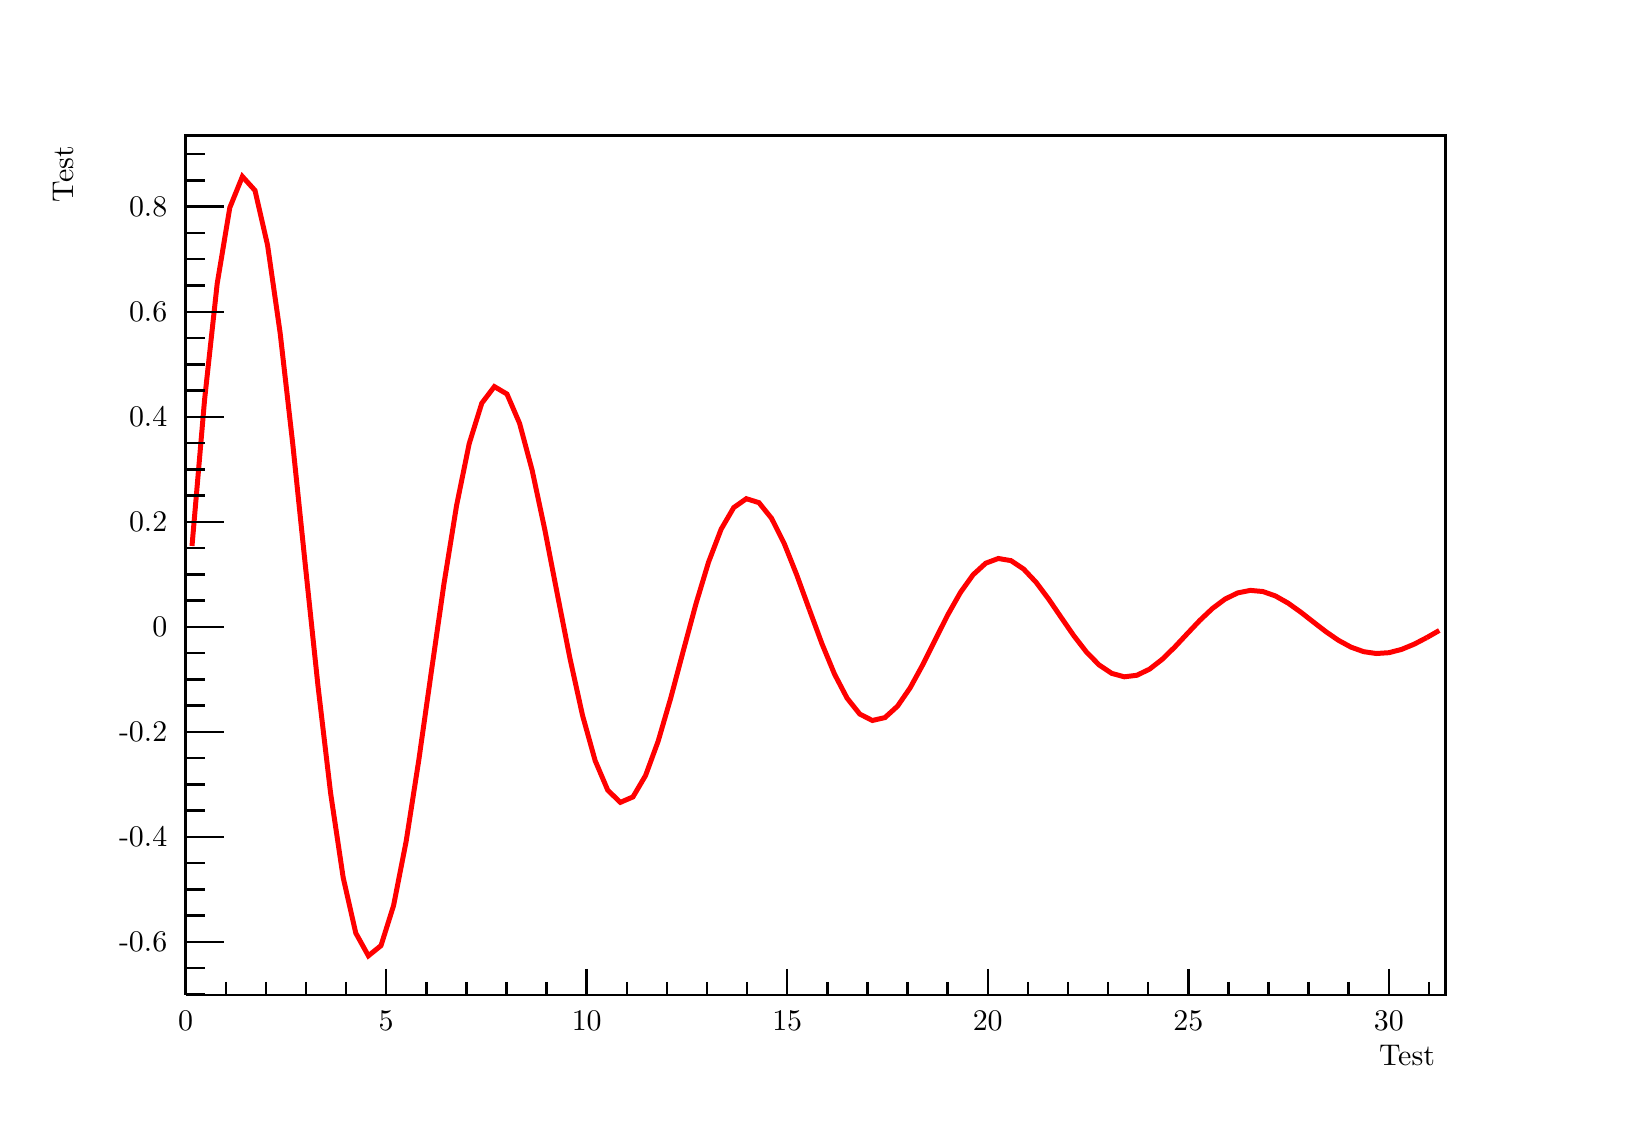
\begin{tikzpicture}
\def\CheckTikzLibraryLoaded#1{ \ifcsname tikz@library@#1@loaded\endcsname \else \PackageWarning{tikz}{usetikzlibrary{#1} is missing in the preamble.} \fi }
\CheckTikzLibraryLoaded{patterns}
\CheckTikzLibraryLoaded{plotmarks}
\pgfdeclareplotmark{cross} {
\pgfpathmoveto{\pgfpoint{-0.3\pgfplotmarksize}{\pgfplotmarksize}}
\pgfpathlineto{\pgfpoint{+0.3\pgfplotmarksize}{\pgfplotmarksize}}
\pgfpathlineto{\pgfpoint{+0.3\pgfplotmarksize}{0.3\pgfplotmarksize}}
\pgfpathlineto{\pgfpoint{+1\pgfplotmarksize}{0.3\pgfplotmarksize}}
\pgfpathlineto{\pgfpoint{+1\pgfplotmarksize}{-0.3\pgfplotmarksize}}
\pgfpathlineto{\pgfpoint{+0.3\pgfplotmarksize}{-0.3\pgfplotmarksize}}
\pgfpathlineto{\pgfpoint{+0.3\pgfplotmarksize}{-1.\pgfplotmarksize}}
\pgfpathlineto{\pgfpoint{-0.3\pgfplotmarksize}{-1.\pgfplotmarksize}}
\pgfpathlineto{\pgfpoint{-0.3\pgfplotmarksize}{-0.3\pgfplotmarksize}}
\pgfpathlineto{\pgfpoint{-1.\pgfplotmarksize}{-0.3\pgfplotmarksize}}
\pgfpathlineto{\pgfpoint{-1.\pgfplotmarksize}{0.3\pgfplotmarksize}}
\pgfpathlineto{\pgfpoint{-0.3\pgfplotmarksize}{0.3\pgfplotmarksize}}
\pgfpathclose
\pgfusepathqstroke
}
\pgfdeclareplotmark{cross*} {
\pgfpathmoveto{\pgfpoint{-0.3\pgfplotmarksize}{\pgfplotmarksize}}
\pgfpathlineto{\pgfpoint{+0.3\pgfplotmarksize}{\pgfplotmarksize}}
\pgfpathlineto{\pgfpoint{+0.3\pgfplotmarksize}{0.3\pgfplotmarksize}}
\pgfpathlineto{\pgfpoint{+1\pgfplotmarksize}{0.3\pgfplotmarksize}}
\pgfpathlineto{\pgfpoint{+1\pgfplotmarksize}{-0.3\pgfplotmarksize}}
\pgfpathlineto{\pgfpoint{+0.3\pgfplotmarksize}{-0.3\pgfplotmarksize}}
\pgfpathlineto{\pgfpoint{+0.3\pgfplotmarksize}{-1.\pgfplotmarksize}}
\pgfpathlineto{\pgfpoint{-0.3\pgfplotmarksize}{-1.\pgfplotmarksize}}
\pgfpathlineto{\pgfpoint{-0.3\pgfplotmarksize}{-0.3\pgfplotmarksize}}
\pgfpathlineto{\pgfpoint{-1.\pgfplotmarksize}{-0.3\pgfplotmarksize}}
\pgfpathlineto{\pgfpoint{-1.\pgfplotmarksize}{0.3\pgfplotmarksize}}
\pgfpathlineto{\pgfpoint{-0.3\pgfplotmarksize}{0.3\pgfplotmarksize}}
\pgfpathclose
\pgfusepathqfillstroke
}
\pgfdeclareplotmark{newstar} {
\pgfpathmoveto{\pgfqpoint{0pt}{\pgfplotmarksize}}
\pgfpathlineto{\pgfqpointpolar{44}{0.5\pgfplotmarksize}}
\pgfpathlineto{\pgfqpointpolar{18}{\pgfplotmarksize}}
\pgfpathlineto{\pgfqpointpolar{-20}{0.5\pgfplotmarksize}}
\pgfpathlineto{\pgfqpointpolar{-54}{\pgfplotmarksize}}
\pgfpathlineto{\pgfqpointpolar{-90}{0.5\pgfplotmarksize}}
\pgfpathlineto{\pgfqpointpolar{234}{\pgfplotmarksize}}
\pgfpathlineto{\pgfqpointpolar{198}{0.5\pgfplotmarksize}}
\pgfpathlineto{\pgfqpointpolar{162}{\pgfplotmarksize}}
\pgfpathlineto{\pgfqpointpolar{134}{0.5\pgfplotmarksize}}
\pgfpathclose
\pgfusepathqstroke
}
\pgfdeclareplotmark{newstar*} {
\pgfpathmoveto{\pgfqpoint{0pt}{\pgfplotmarksize}}
\pgfpathlineto{\pgfqpointpolar{44}{0.5\pgfplotmarksize}}
\pgfpathlineto{\pgfqpointpolar{18}{\pgfplotmarksize}}
\pgfpathlineto{\pgfqpointpolar{-20}{0.5\pgfplotmarksize}}
\pgfpathlineto{\pgfqpointpolar{-54}{\pgfplotmarksize}}
\pgfpathlineto{\pgfqpointpolar{-90}{0.5\pgfplotmarksize}}
\pgfpathlineto{\pgfqpointpolar{234}{\pgfplotmarksize}}
\pgfpathlineto{\pgfqpointpolar{198}{0.5\pgfplotmarksize}}
\pgfpathlineto{\pgfqpointpolar{162}{\pgfplotmarksize}}
\pgfpathlineto{\pgfqpointpolar{134}{0.5\pgfplotmarksize}}
\pgfpathclose
\pgfusepathqfillstroke
}
\definecolor{c}{rgb}{1,1,1};
\draw [color=c, fill=c] (0,0) rectangle (20,13.639);
\draw [color=c, fill=c] (2,1.3639) rectangle (18,12.2751);
\definecolor{c}{rgb}{0,0,0};
\draw [c,line width=0.9] (2,1.3639) -- (2,12.2751) -- (18,12.2751) -- (18,1.3639) -- (2,1.3639);
\definecolor{c}{rgb}{1,0,0};
\draw [c,line width=1.8] (2.08,7.0633) -- (2.24,8.92486) -- (2.4,10.3963) -- (2.56,11.3603) -- (2.72,11.7555) -- (2.88,11.5786) -- (3.04,10.8814) -- (3.2,9.76247) -- (3.36,8.3546) -- (3.52,6.81033) -- (3.68,5.28592) -- (3.84,3.92623) -- (4,2.85151)
 -- (4.16,2.14738) -- (4.32,1.85873) -- (4.48,1.98793) -- (4.64,2.49715) -- (4.8,3.31444) -- (4.96,4.34275) -- (5.12,5.47069) -- (5.28,6.58413) -- (5.44,7.57725) -- (5.6,8.36223) -- (5.76,8.87653) -- (5.92,9.08735) -- (6.08,8.99299) -- (6.24,8.62105)
 -- (6.4,8.0241) -- (6.56,7.27302) -- (6.72,6.44917) -- (6.88,5.63591) -- (7.04,4.91054) -- (7.2,4.33719) -- (7.36,3.96154) -- (7.52,3.80755) -- (7.68,3.87648) -- (7.84,4.14814) -- (8,4.58415) -- (8.16,5.13274) -- (8.32,5.73449) -- (8.48,6.32849) --
 (8.64,6.85831) -- (8.8,7.27709) -- (8.96,7.55146) -- (9.12,7.66393) -- (9.28,7.61359) -- (9.44,7.41517) -- (9.6,7.0967) -- (9.76,6.69601) -- (9.92,6.25649);
\draw [c,line width=1.8] (9.92,6.25649) -- (10.08,5.82263) -- (10.24,5.43565) -- (10.4,5.12977) -- (10.56,4.92937) -- (10.72,4.84722) -- (10.88,4.88399) -- (11.04,5.02892) -- (11.2,5.26153) -- (11.36,5.5542) -- (11.52,5.87522) -- (11.68,6.19211) --
 (11.84,6.47476) -- (12,6.69818) -- (12.16,6.84455) -- (12.32,6.90455) -- (12.48,6.8777) -- (12.64,6.77184) -- (12.8,6.60194) -- (12.96,6.38818) -- (13.12,6.1537) -- (13.28,5.92224) -- (13.44,5.71579) -- (13.6,5.55261) -- (13.76,5.4457) --
 (13.92,5.40187) -- (14.08,5.42149) -- (14.24,5.49881) -- (14.4,5.6229) -- (14.56,5.77904) -- (14.72,5.9503) -- (14.88,6.11936) -- (15.04,6.27015) -- (15.2,6.38934) -- (15.36,6.46742) -- (15.52,6.49944) -- (15.68,6.48511) -- (15.84,6.42863) --
 (16,6.338) -- (16.16,6.22395) -- (16.32,6.09886) -- (16.48,5.97538) -- (16.64,5.86525) -- (16.8,5.77819) -- (16.96,5.72115) -- (17.12,5.69777) -- (17.28,5.70824) -- (17.44,5.74949) -- (17.6,5.81569) -- (17.76,5.89898);
\draw [c,line width=1.8] (17.76,5.89898) -- (17.92,5.99035);
\definecolor{c}{rgb}{0,0,0};
\draw [c,line width=0.9] (2,1.3639) -- (18,1.3639);
\draw [c,line width=0.9] (2,1.69123) -- (2,1.3639);
\draw [c,line width=0.9] (2.5093,1.52756) -- (2.5093,1.3639);
\draw [c,line width=0.9] (3.01859,1.52756) -- (3.01859,1.3639);
\draw [c,line width=0.9] (3.52789,1.52756) -- (3.52789,1.3639);
\draw [c,line width=0.9] (4.03718,1.52756) -- (4.03718,1.3639);
\draw [c,line width=0.9] (4.54648,1.69123) -- (4.54648,1.3639);
\draw [c,line width=0.9] (5.05578,1.52756) -- (5.05578,1.3639);
\draw [c,line width=0.9] (5.56507,1.52756) -- (5.56507,1.3639);
\draw [c,line width=0.9] (6.07437,1.52756) -- (6.07437,1.3639);
\draw [c,line width=0.9] (6.58366,1.52756) -- (6.58366,1.3639);
\draw [c,line width=0.9] (7.09296,1.69123) -- (7.09296,1.3639);
\draw [c,line width=0.9] (7.60225,1.52756) -- (7.60225,1.3639);
\draw [c,line width=0.9] (8.11155,1.52756) -- (8.11155,1.3639);
\draw [c,line width=0.9] (8.62085,1.52756) -- (8.62085,1.3639);
\draw [c,line width=0.9] (9.13014,1.52756) -- (9.13014,1.3639);
\draw [c,line width=0.9] (9.63944,1.69123) -- (9.63944,1.3639);
\draw [c,line width=0.9] (10.1487,1.52756) -- (10.1487,1.3639);
\draw [c,line width=0.9] (10.658,1.52756) -- (10.658,1.3639);
\draw [c,line width=0.9] (11.1673,1.52756) -- (11.1673,1.3639);
\draw [c,line width=0.9] (11.6766,1.52756) -- (11.6766,1.3639);
\draw [c,line width=0.9] (12.1859,1.69123) -- (12.1859,1.3639);
\draw [c,line width=0.9] (12.6952,1.52756) -- (12.6952,1.3639);
\draw [c,line width=0.9] (13.2045,1.52756) -- (13.2045,1.3639);
\draw [c,line width=0.9] (13.7138,1.52756) -- (13.7138,1.3639);
\draw [c,line width=0.9] (14.2231,1.52756) -- (14.2231,1.3639);
\draw [c,line width=0.9] (14.7324,1.69123) -- (14.7324,1.3639);
\draw [c,line width=0.9] (15.2417,1.52756) -- (15.2417,1.3639);
\draw [c,line width=0.9] (15.751,1.52756) -- (15.751,1.3639);
\draw [c,line width=0.9] (16.2603,1.52756) -- (16.2603,1.3639);
\draw [c,line width=0.9] (16.7696,1.52756) -- (16.7696,1.3639);
\draw [c,line width=0.9] (17.2789,1.69123) -- (17.2789,1.3639);
\draw [c,line width=0.9] (17.2789,1.69123) -- (17.2789,1.3639);
\draw [c,line width=0.9] (17.7882,1.52756) -- (17.7882,1.3639);
\draw [anchor=base] (2,0.913811) node[scale=1.08185, color=c, rotate=0]{0};
\draw [anchor=base] (4.54648,0.913811) node[scale=1.08185, color=c, rotate=0]{5};
\draw [anchor=base] (7.09296,0.913811) node[scale=1.08185, color=c, rotate=0]{10};
\draw [anchor=base] (9.63944,0.913811) node[scale=1.08185, color=c, rotate=0]{15};
\draw [anchor=base] (12.1859,0.913811) node[scale=1.08185, color=c, rotate=0]{20};
\draw [anchor=base] (14.7324,0.913811) node[scale=1.08185, color=c, rotate=0]{25};
\draw [anchor=base] (17.2789,0.913811) node[scale=1.08185, color=c, rotate=0]{30};
\draw [anchor= east] (18,0.600115) node[scale=1.08185, color=c, rotate=0]{Test};
\draw [c,line width=0.9] (2,1.3639) -- (2,12.2751);
\draw [c,line width=0.9] (2.48,2.03418) -- (2,2.03418);
\draw [c,line width=0.9] (2.24,2.36768) -- (2,2.36768);
\draw [c,line width=0.9] (2.24,2.70118) -- (2,2.70118);
\draw [c,line width=0.9] (2.24,3.03468) -- (2,3.03468);
\draw [c,line width=0.9] (2.48,3.36817) -- (2,3.36817);
\draw [c,line width=0.9] (2.24,3.70167) -- (2,3.70167);
\draw [c,line width=0.9] (2.24,4.03517) -- (2,4.03517);
\draw [c,line width=0.9] (2.24,4.36867) -- (2,4.36867);
\draw [c,line width=0.9] (2.48,4.70216) -- (2,4.70216);
\draw [c,line width=0.9] (2.24,5.03566) -- (2,5.03566);
\draw [c,line width=0.9] (2.24,5.36916) -- (2,5.36916);
\draw [c,line width=0.9] (2.24,5.70266) -- (2,5.70266);
\draw [c,line width=0.9] (2.48,6.03615) -- (2,6.03615);
\draw [c,line width=0.9] (2.24,6.36965) -- (2,6.36965);
\draw [c,line width=0.9] (2.24,6.70315) -- (2,6.70315);
\draw [c,line width=0.9] (2.24,7.03665) -- (2,7.03665);
\draw [c,line width=0.9] (2.48,7.37014) -- (2,7.37014);
\draw [c,line width=0.9] (2.24,7.70364) -- (2,7.70364);
\draw [c,line width=0.9] (2.24,8.03714) -- (2,8.03714);
\draw [c,line width=0.9] (2.24,8.37064) -- (2,8.37064);
\draw [c,line width=0.9] (2.48,8.70413) -- (2,8.70413);
\draw [c,line width=0.9] (2.24,9.03763) -- (2,9.03763);
\draw [c,line width=0.9] (2.24,9.37113) -- (2,9.37113);
\draw [c,line width=0.9] (2.24,9.70463) -- (2,9.70463);
\draw [c,line width=0.9] (2.48,10.0381) -- (2,10.0381);
\draw [c,line width=0.9] (2.24,10.3716) -- (2,10.3716);
\draw [c,line width=0.9] (2.24,10.7051) -- (2,10.7051);
\draw [c,line width=0.9] (2.24,11.0386) -- (2,11.0386);
\draw [c,line width=0.9] (2.48,11.3721) -- (2,11.3721);
\draw [c,line width=0.9] (2.48,2.03418) -- (2,2.03418);
\draw [c,line width=0.9] (2.24,1.70069) -- (2,1.70069);
\draw [c,line width=0.9] (2.24,1.36719) -- (2,1.36719);
\draw [c,line width=0.9] (2.48,11.3721) -- (2,11.3721);
\draw [c,line width=0.9] (2.24,11.7056) -- (2,11.7056);
\draw [c,line width=0.9] (2.24,12.0391) -- (2,12.0391);
\draw [anchor= east] (1.9,2.03418) node[scale=1.08185, color=c, rotate=0]{-0.6};
\draw [anchor= east] (1.9,3.36817) node[scale=1.08185, color=c, rotate=0]{-0.4};
\draw [anchor= east] (1.9,4.70216) node[scale=1.08185, color=c, rotate=0]{-0.2};
\draw [anchor= east] (1.9,6.03615) node[scale=1.08185, color=c, rotate=0]{0};
\draw [anchor= east] (1.9,7.37014) node[scale=1.08185, color=c, rotate=0]{0.2};
\draw [anchor= east] (1.9,8.70413) node[scale=1.08185, color=c, rotate=0]{0.4};
\draw [anchor= east] (1.9,10.0381) node[scale=1.08185, color=c, rotate=0]{0.6};
\draw [anchor= east] (1.9,11.3721) node[scale=1.08185, color=c, rotate=0]{0.8};
\draw [anchor= east] (0.440401,12.2751) node[scale=1.08185, color=c, rotate=90]{Test};
\end{tikzpicture}
%\end{document}
